\documentclass[11pt,a4paper]{article}
\usepackage[utf8]{inputenc}
\usepackage[T1]{fontenc}
\usepackage[french]{babel}
\usepackage[margin=2.2cm]{geometry}
\usepackage{graphicx,booktabs,float,xcolor,hyperref}
\hypersetup{hidelinks,pdftitle={Conclusion personnelle de synthèse - Cartographie et localisation},pdfauthor={Houssam MAKHLOUK}}
\setlength{\parskip}{0.45em}
\setlength{\parindent}{0pt}
\renewcommand{\arraystretch}{1.18}

\begin{document}
\hypersetup{pageanchor=false}
\begin{titlepage}
\centering
\vspace*{1.5cm}
{\Large\bfseries EIGSI\par}
\vspace{0.35cm}
{\large Année universitaire 2026/2027\par}
\vspace{2cm}
{\color{blue!45!black}\rule{0.88\textwidth}{1.2pt}\par}
\vspace{0.65cm}
{\Huge\bfseries Conclusion personnelle\par}
\vspace{0.3cm}
{\LARGE\bfseries Synthèse du module de cartographie\par}
{\LARGE\bfseries et localisation en robotique mobile\par}
\vspace{0.65cm}
{\color{blue!45!black}\rule{0.88\textwidth}{1.2pt}\par}
\vspace{1cm}
{\large Extraction LiDAR, cartes 2D, scan matching et premiers pas en SLAM\par}
\vfill
{\large Houssam MAKHLOUK\par}
{\large Étudiant à EIGSI\par}
\vspace*{1cm}
\end{titlepage}

\hypersetup{pageanchor=true}
\tableofcontents
\clearpage

\section{Ce que j'ai réalisé dans le module}
Au cours des trois journées de travaux pratiques, j'ai suivi une chaîne complète, depuis les mesures brutes du LiDAR LD06 jusqu'à une carte construite à partir de plusieurs positions du capteur. Le premier TP m'a fait acquérir, afficher et représenter des scans. Le deuxième m'a conduit à estimer la pose d'un scan par rapport à trois types de références. Le troisième a relié ces deux parties dans un traitement incrémental : chaque nouveau scan est localisé par rapport à la carte courante, puis ajouté à celle-ci si le recalage est jugé suffisamment cohérent.

Les documentations fournies par le professeur m'ont aidé à comprendre et à organiser ce travail. Les supports sur la construction d'une grid map, la carte vectorielle, l'expression de la pose du robot et le scan matching ont donné un cadre pour passer des équations aux programmes. Ils ont notamment clarifié la différence entre une cellule traversée par un rayon et une cellule d'impact, ainsi que le rôle de la rotation et de la translation dans le changement de repère. J'ai ensuite dû choisir des paramètres, vérifier les résultats sur mes propres scans et analyser les cas où les méthodes ne concordaient pas.

\section{TP1 : acquisition, visualisation et cartographie}
\subsection{Extraction et affichage des scans}
J'ai acquis quatre scans réels pour le TP1, soit 1\,821 points au total. Les fichiers CSV conservent l'angle, la distance, l'intensité et les coordonnées cartésiennes locales. J'ai vérifié les unités : les distances sont enregistrées en millimètres, alors que les figures et les poses utilisent des mètres. J'ai aussi conservé la convention de signe de l'axe $Y$ présente dans les CSV pour éviter d'inverser la salle lors de la conversion.

Le visualiseur Python affiche les scans simultanément avec des couleurs distinctes. Je peux modifier séparément la position $(x,y)$ et l'orientation $\theta$ de chaque scan, enregistrer les poses, puis exporter les points transformés. Le visualiseur HTML permet également de déposer des CSV dans le navigateur, d'examiner le nuage, de corriger les poses et d'exporter une figure. Ces deux interfaces m'ont permis de voir immédiatement si des murs communs se superposaient. L'alignement de quatre scans reste une \emph{estimation géométrique} : la coïncidence visuelle des points ne constitue pas une mesure indépendante de la pose réelle du capteur.

\begin{figure}[H]\centering
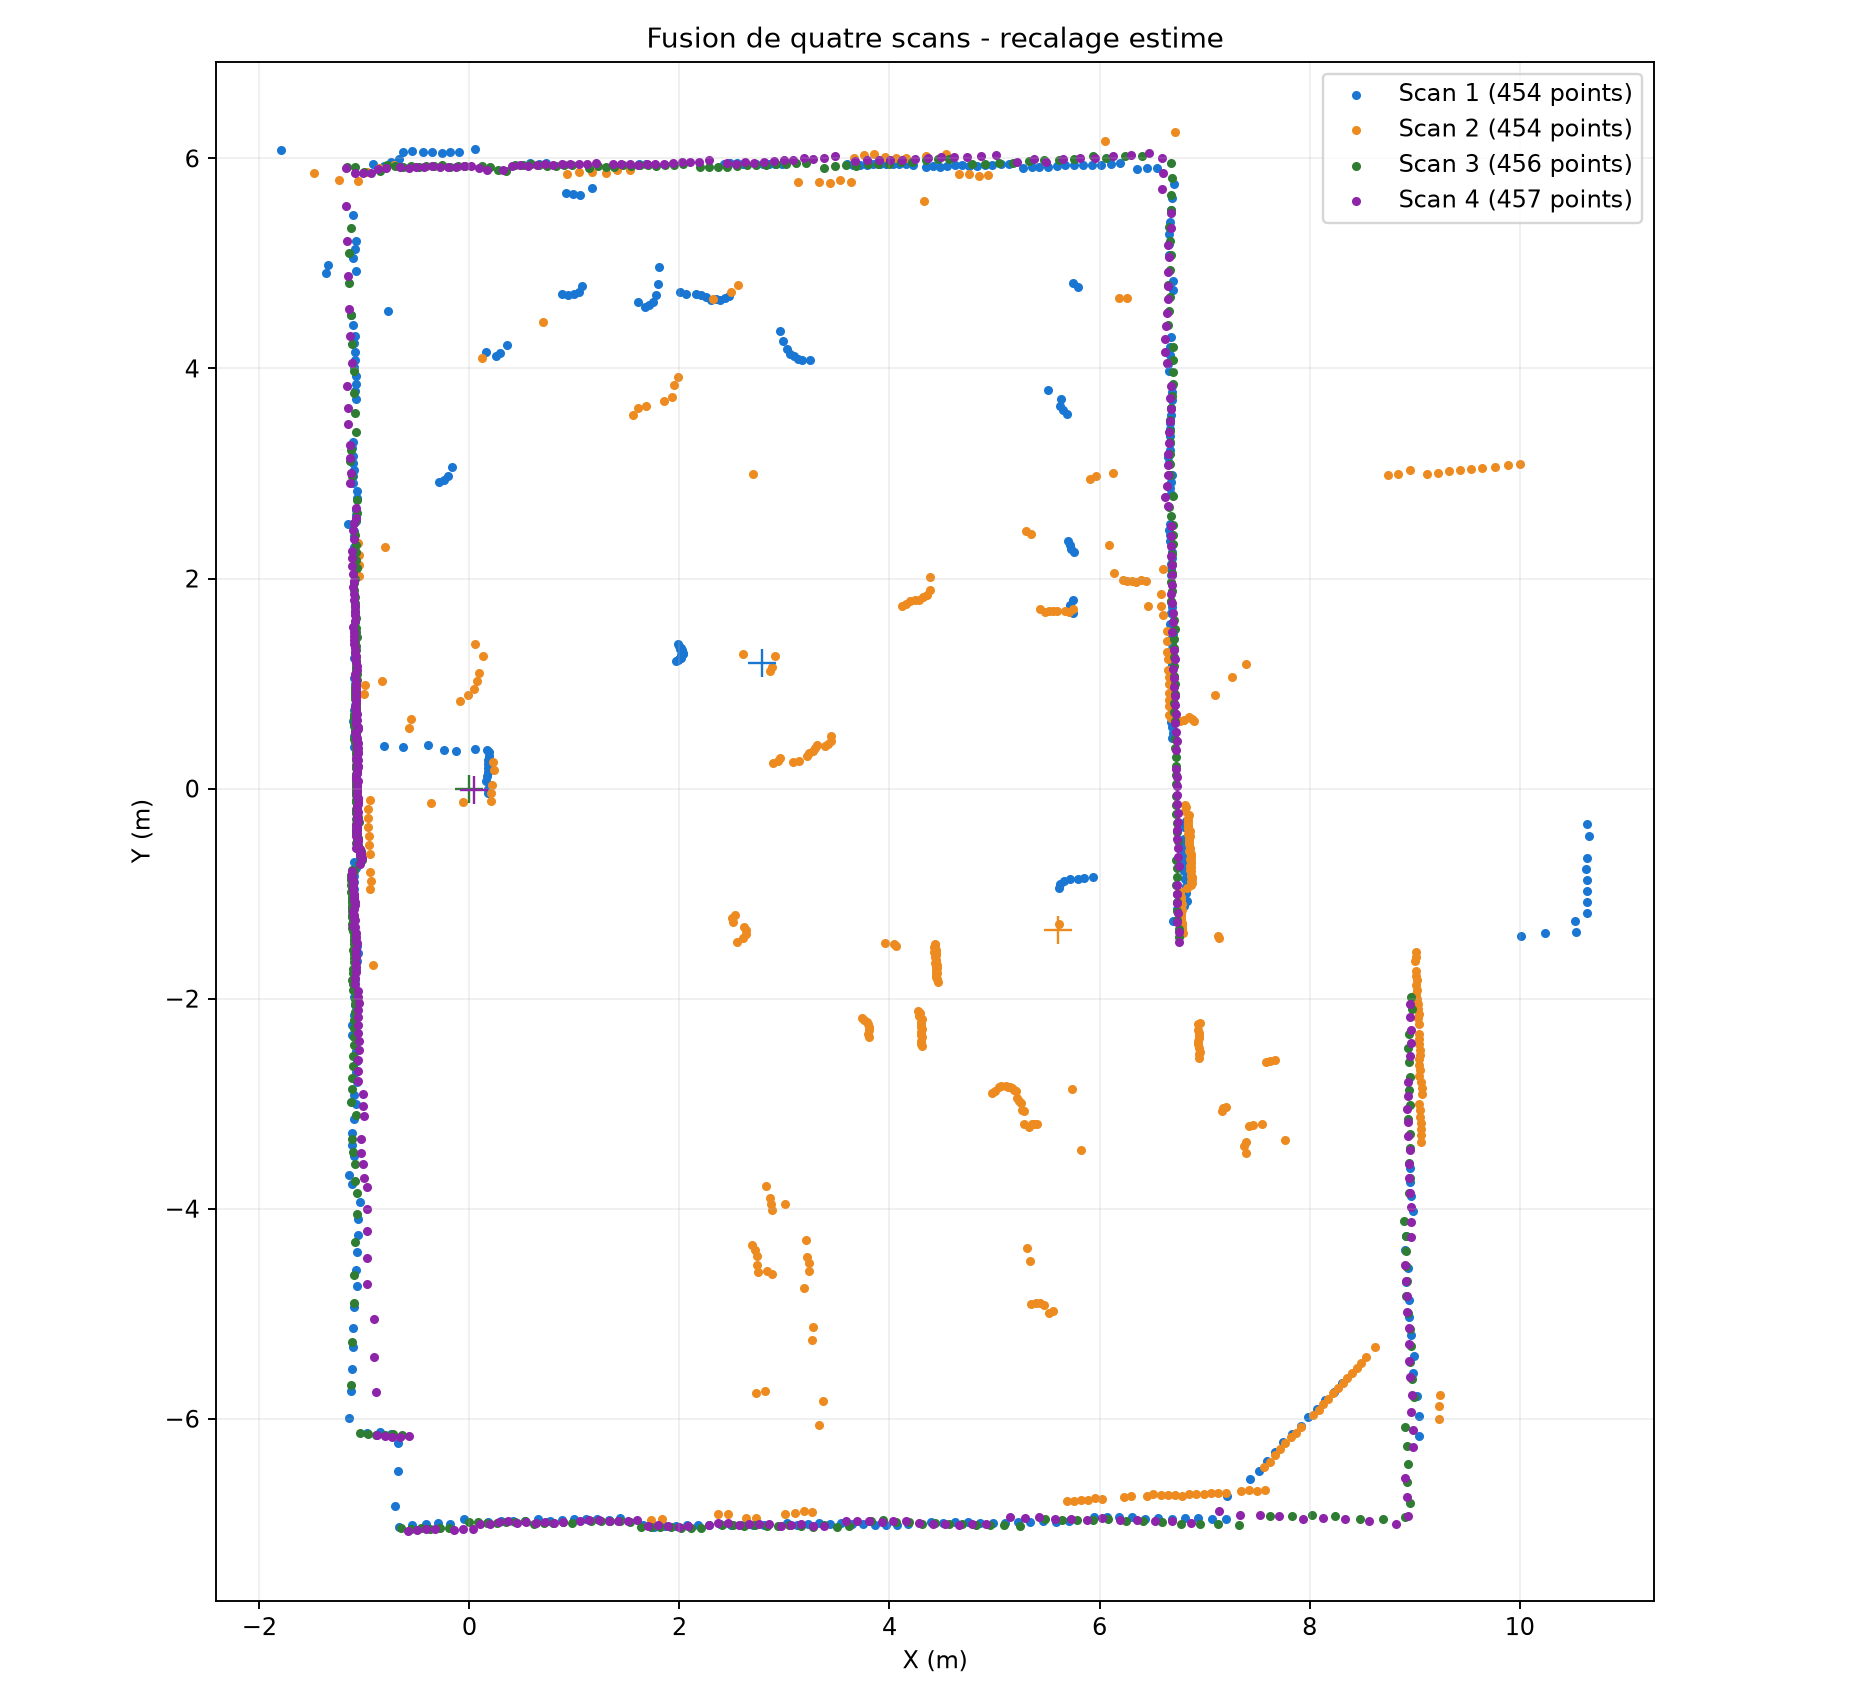
\includegraphics[width=0.88\textwidth]{../tp1/TP1_4_scans/resultats/fusion_4_scans.png}
\caption{Visualisation et fusion estimée des quatre acquisitions du TP1. Les couleurs distinguent les scans.}
\end{figure}

\subsection{Grid map : choix, fonctionnement et résultat}
J'ai choisi une grille de résolution 5 cm pour conserver le détail des obstacles tout en gardant une taille de fichier et un temps de calcul raisonnables. Chaque cellule commence dans l'état \emph{inconnu}. Pour chaque mesure, le programme place d'abord l'origine et le point d'impact dans le repère global. Il parcourt ensuite les cellules entre ces deux points par l'algorithme de Bresenham : les cellules traversées sont marquées \emph{libres}, puis la cellule d'impact est marquée \emph{occupée}. La même carte peut être actualisée par les scans suivants avec leurs poses respectives. La grille finale du TP1 contient $288\times270$ cellules.

\begin{figure}[H]\centering
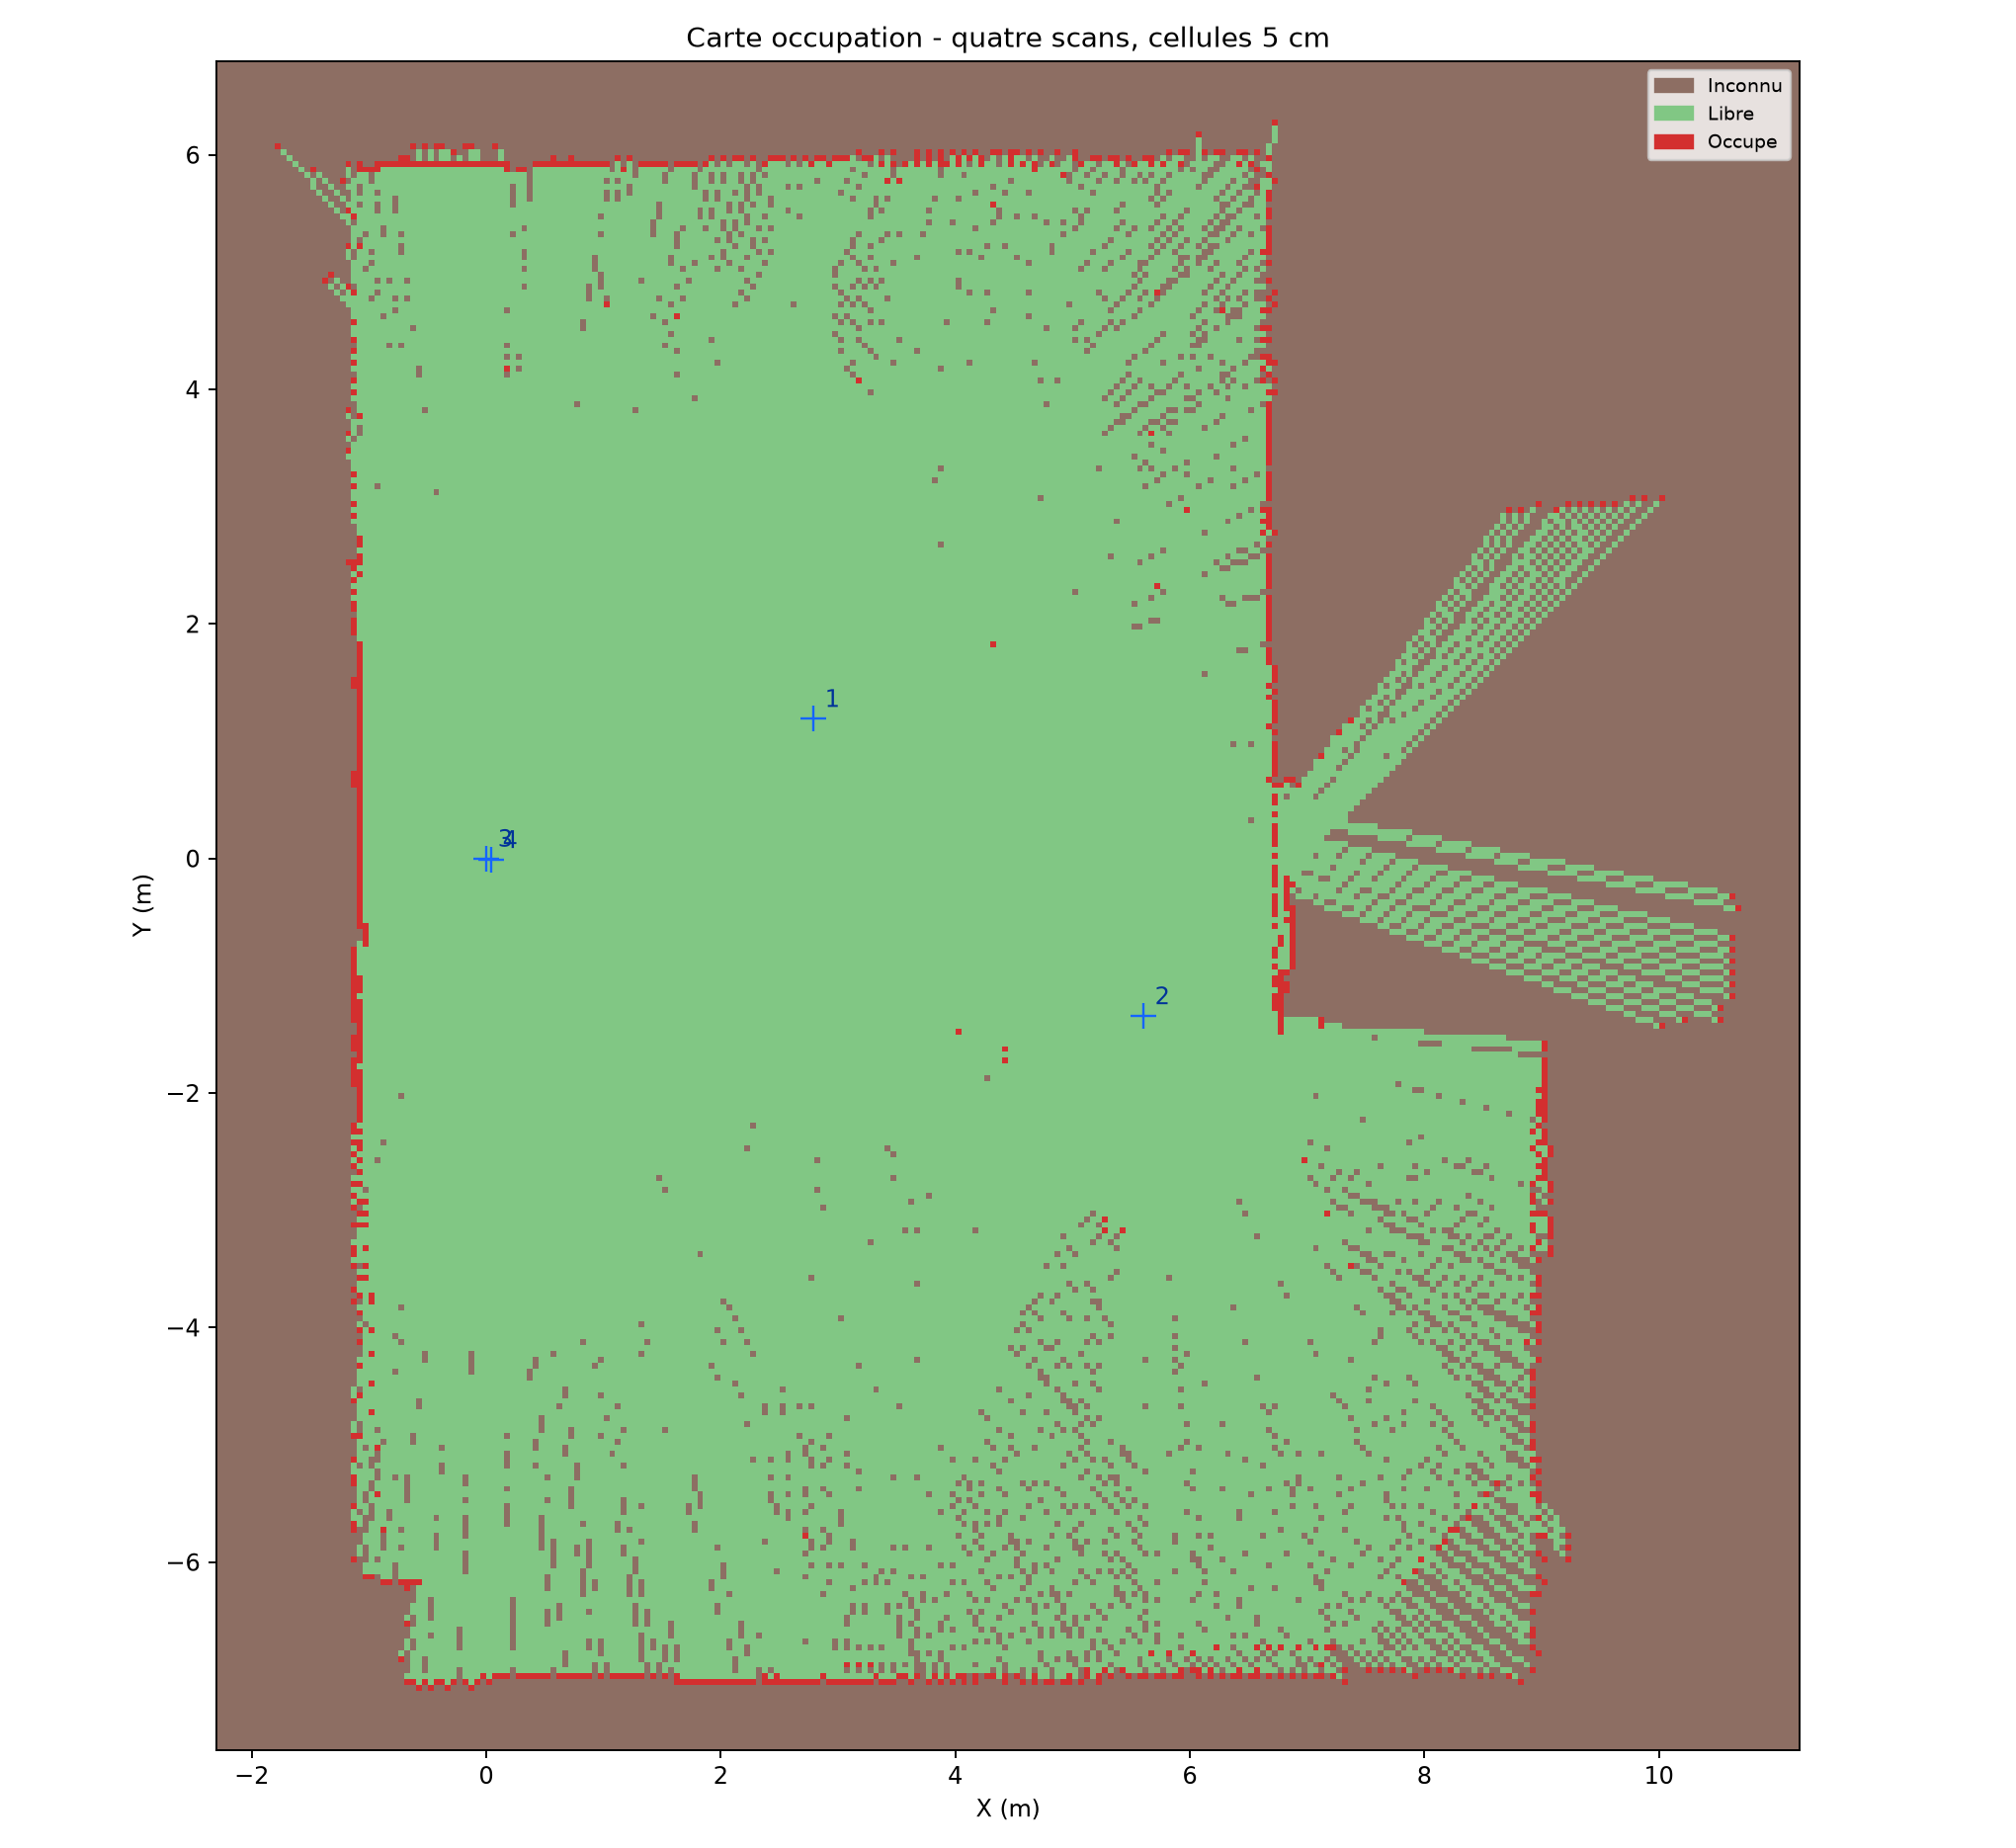
\includegraphics[width=0.81\textwidth]{../tp1/TP1_4_scans/resultats/grid_map_finale.png}
\caption{Carte d'occupation obtenue à partir des quatre scans : espaces observés libres, impacts et zones non observées.}
\end{figure}

Ce résultat rend visibles les zones effectivement traversées par des rayons. Il m'a aussi appris qu'un espace sans point n'est pas nécessairement libre : il peut être masqué ou simplement hors du champ utile. La grille dépend de la qualité des poses ; une petite erreur d'angle décale les murs d'autant plus fortement qu'ils sont éloignés du capteur. Elle décrit une coupe horizontale aux hauteurs d'acquisition, et ne prouve pas à elle seule que toute la pièce a été mesurée.

\subsection{Carte vectorielle et opérations sur les segments}
Pour obtenir une représentation plus compacte, j'ai regroupé les points voisins du scan, ajusté des segments sur les portions suffisamment droites, puis fusionné ceux qui étaient proches en position et en orientation. Les outils géométriques calculent l'angle entre deux segments, leur proximité, leur intersection et la découpe d'un segment traversé par un autre. La découpe ne s'applique que lorsque l'intersection appartient aux deux segments et se trouve strictement à l'intérieur de celui à couper ; les cas colinéaires et les intersections en extrémité sont laissés inchangés. Des tests vérifient ces cas limites.

La carte consolidée du TP1 comporte 38 segments. Elle fait ressortir les longues structures droites et offre un support naturel au scan matching sur segments. Sa limite est qu'un objet courbe, un groupe de personnes ou une série de points interrompus peut être mal représenté par quelques droites. La fusion des segments exige donc des seuils prudents.

\begin{figure}[H]\centering
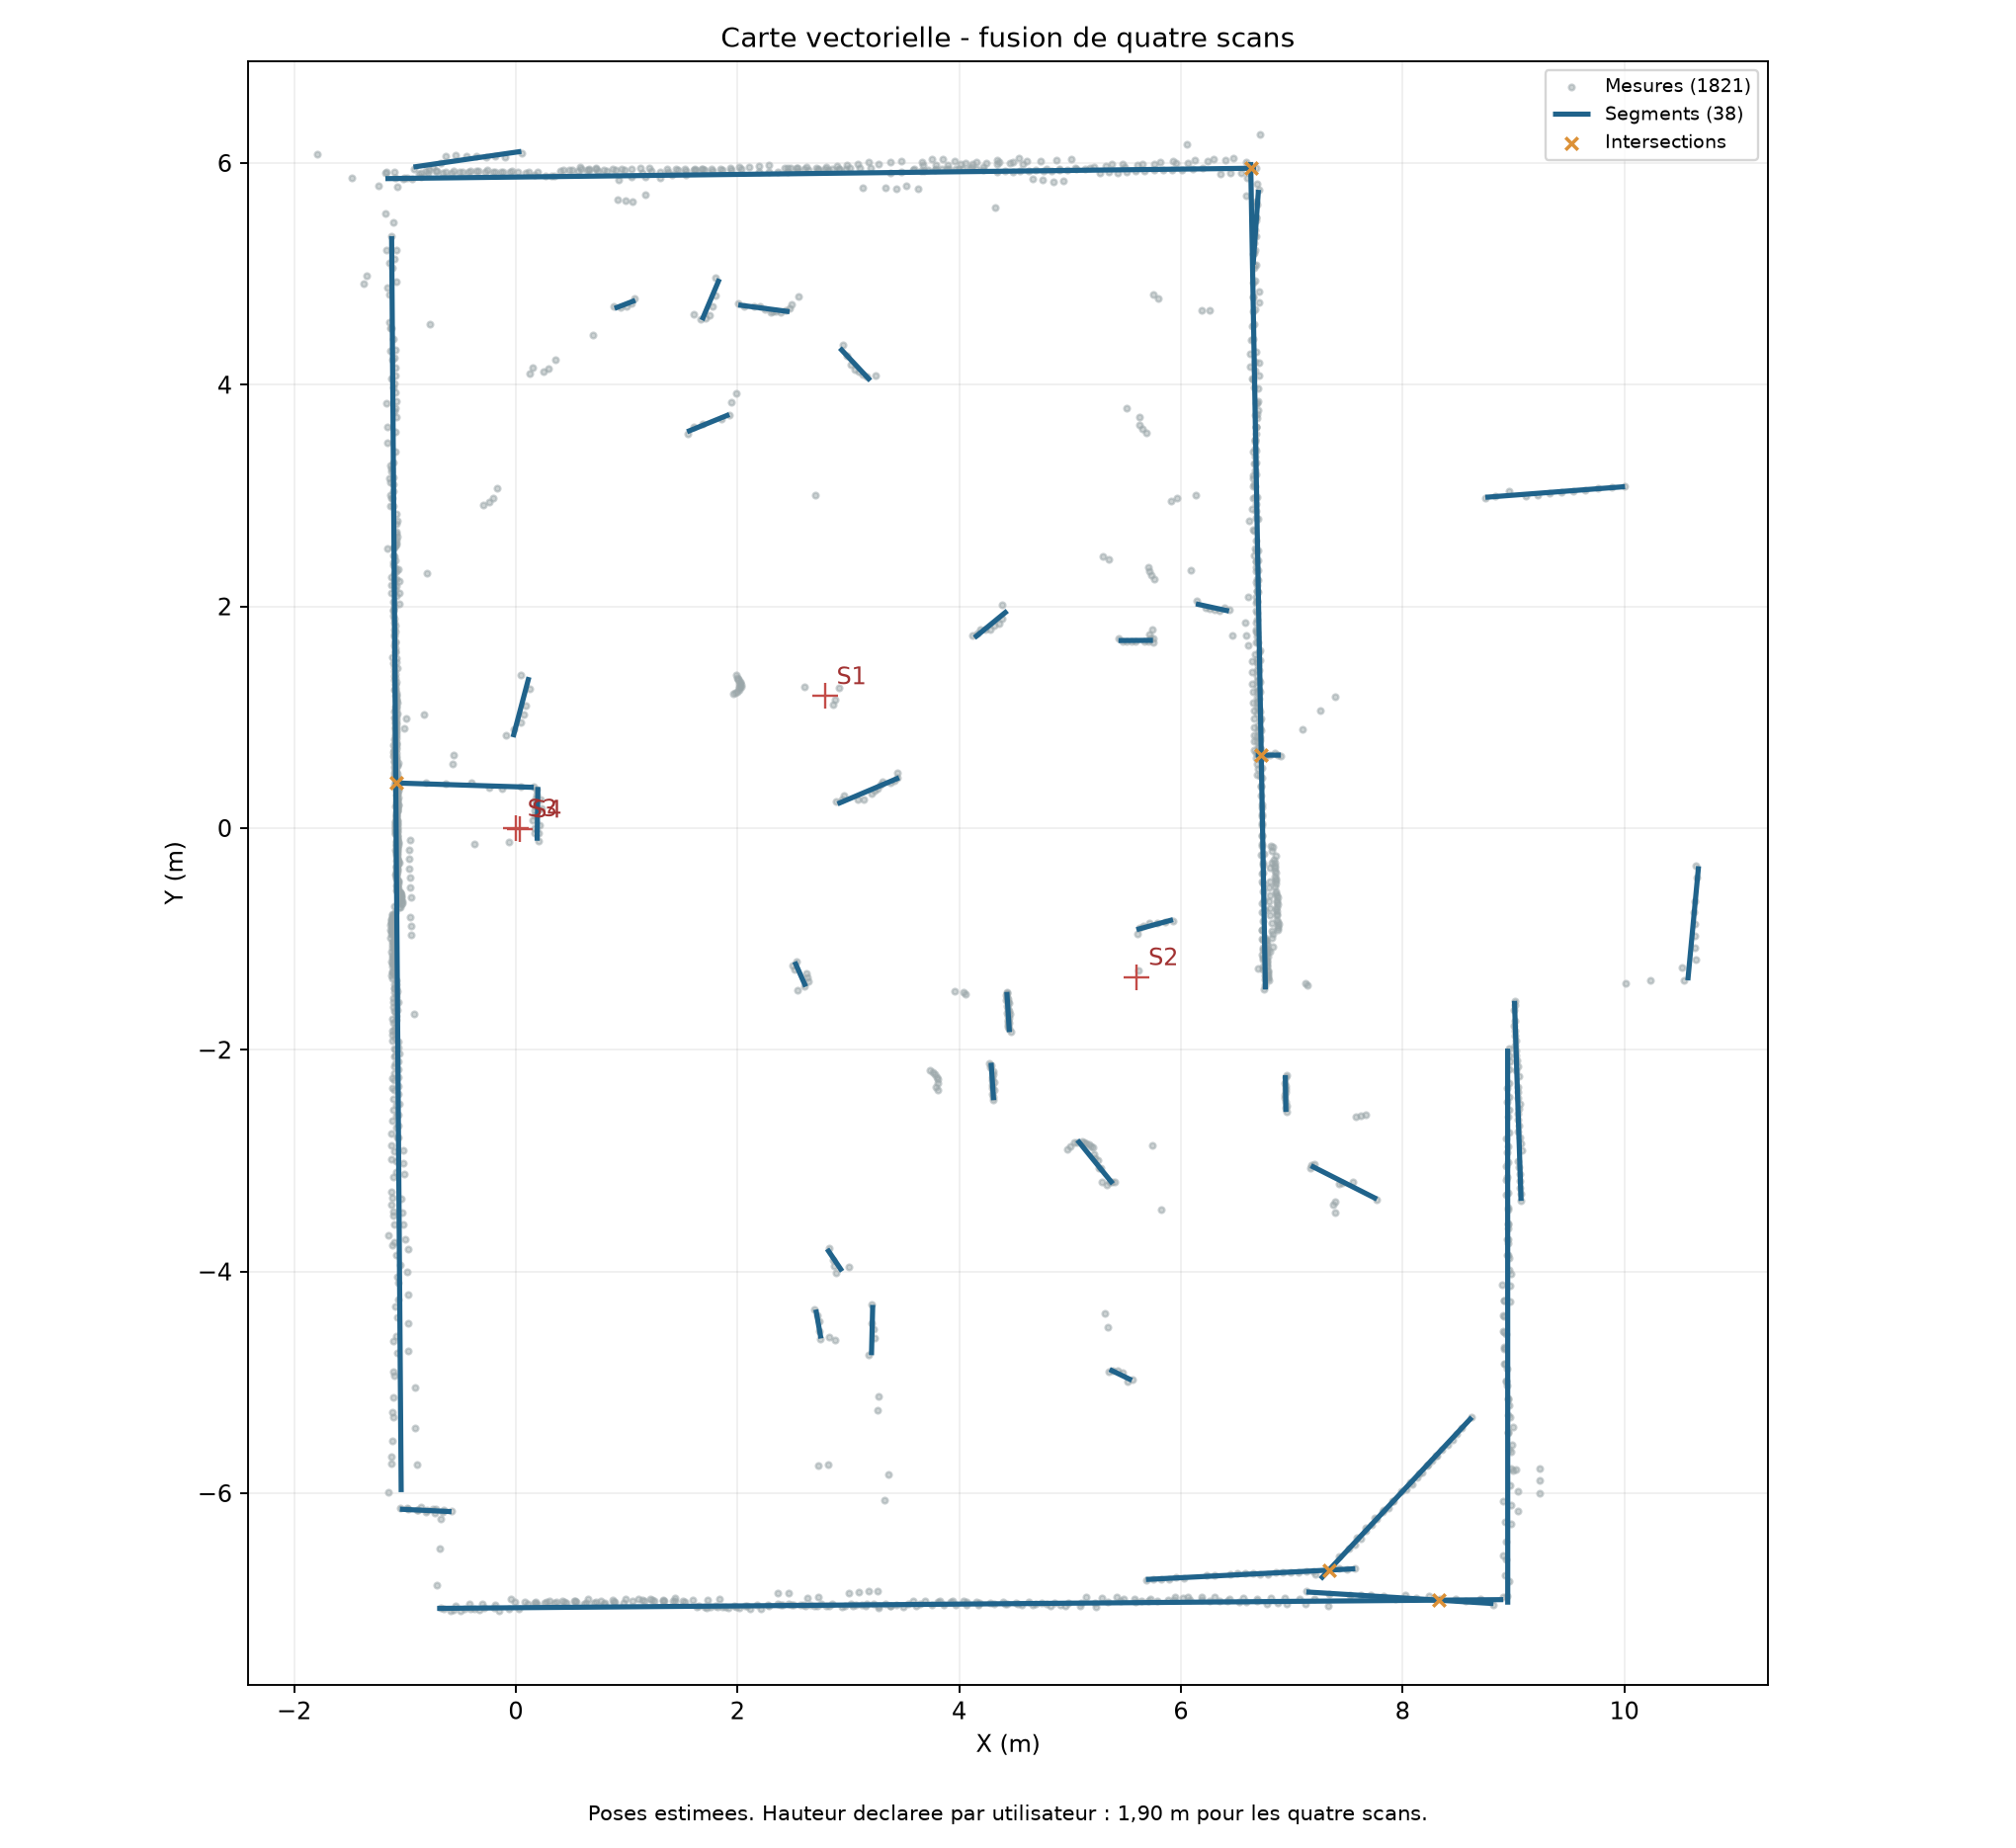
\includegraphics[width=0.81\textwidth]{../tp1/TP1_4_scans/resultats/carte_vectorielle.png}
\caption{Carte vectorielle du TP1, construite par extraction puis consolidation des segments.}
\end{figure}

\section{TP2 : localisation sur trois types de références}
J'ai mis en \oe{}uvre une méthode pour chaque référence demandée. Sur la \textbf{grid map}, la recherche multirésolution déplace et tourne le scan à localiser, puis minimise la distance entre ses impacts et les cellules occupées. Sur la \textbf{carte vectorielle}, une recherche analogue minimise la distance des points transformés aux segments de référence. Pour la \textbf{localisation entre scans}, une recherche grossière fournit une initialisation, suivie d'un recalage ICP sur les points. Les trois méthodes ont été comparées avec les mêmes scans et les mêmes poses de départ.

Le protocole de simulation comporte six scans et dix initialisations par scan, soit 60 essais pour chaque méthode. Une réussite exige une erreur de position d'au plus 0,20 m \emph{et} une erreur angulaire d'au plus $5^\circ$. Les poses vraies sont connues par construction dans cette simulation. La figure et le tableau résument les résultats de cette scène simulée ; ils ne mesurent pas la précision sur le robot réel.

\begin{table}[H]\centering
\begin{tabular}{lrrr}
\toprule
Référence & Erreur moyenne de position & Erreur moyenne d'angle & Temps médian\\
\midrule
Grid map & 0,0145 m & $0,30^\circ$ & 0,075 s\\
Segments & 0,0074 m & $0,375^\circ$ & 0,549 s\\
Scan & 0,0107 m & $0,375^\circ$ & 0,166 s\\
\bottomrule
\end{tabular}
\caption{Comparaison sur la même scène simulée : 60 succès sur 60 essais pour chacune des trois méthodes. Les temps excluent la construction de la référence.}
\end{table}

\begin{figure}[H]\centering
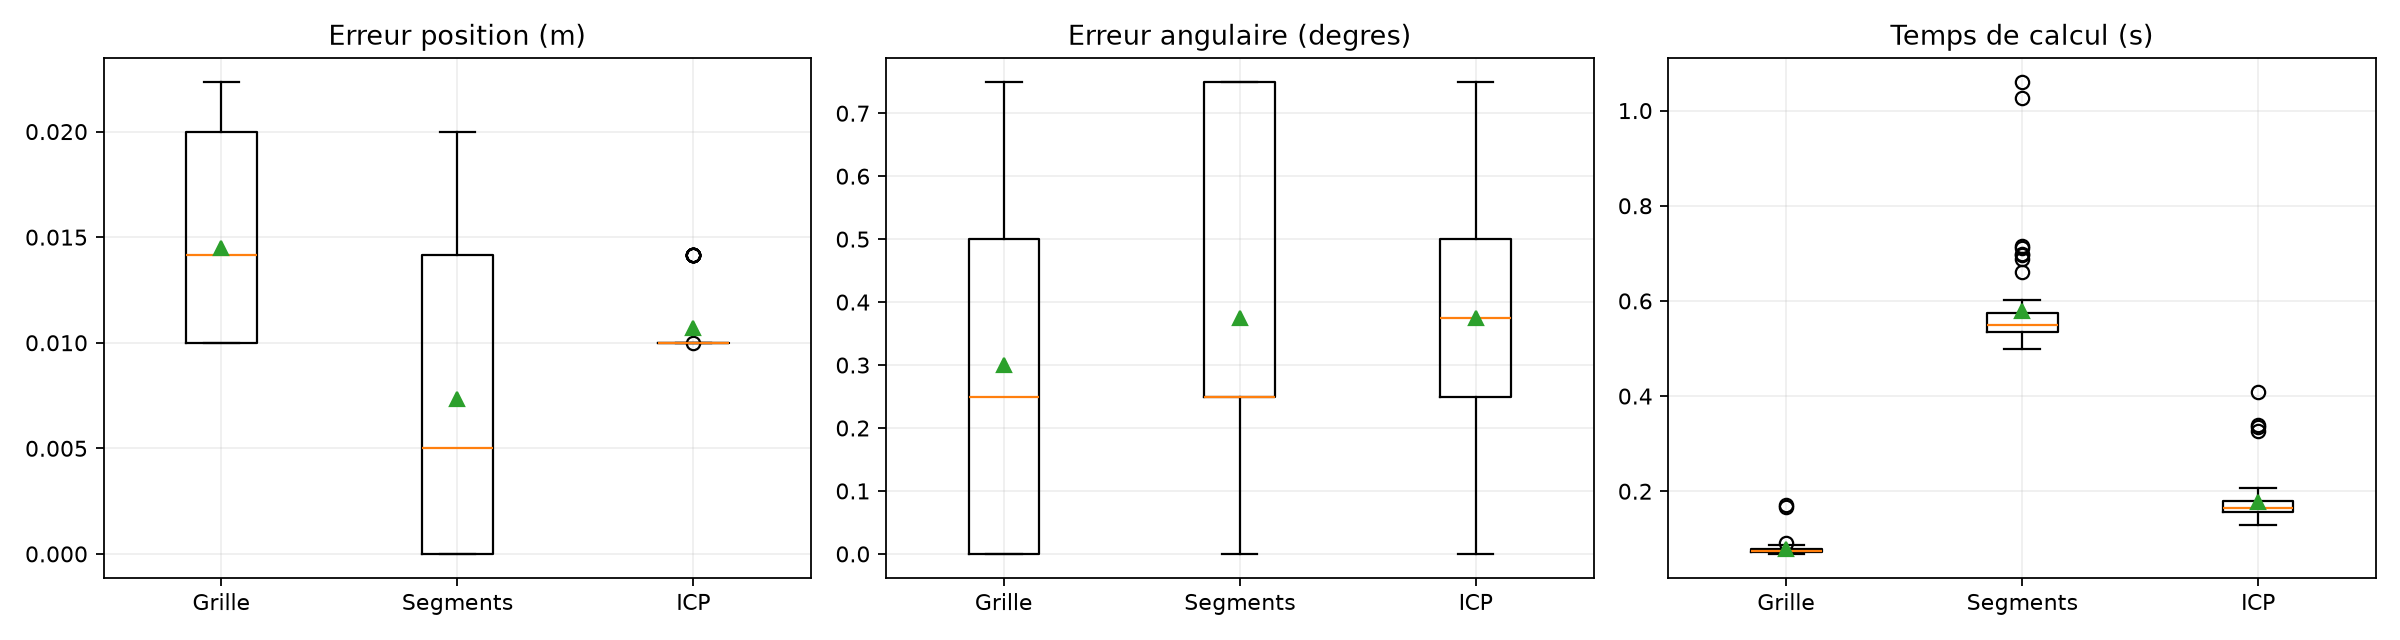
\includegraphics[width=0.88\textwidth]{../tp2/resultats/comparaison_simulation.png}
\caption{Évaluation comparée des trois références sur les scans simulés.}
\end{figure}

J'ai aussi fait varier la pose initiale et testé des CSV réels. Cette seconde étape m'a montré une limite importante : les scores de correspondance peuvent être bons pour plusieurs poses différentes, surtout lorsque des murs se ressemblent ou que les scans se recouvrent peu. Sur la paire réelle N2--N5, les méthodes ne convergent pas toujours vers la même orientation. Les positions et rotations de référence des acquisitions réelles n'ayant pas été relevées avec un instrument indépendant, je ne peux pas calculer une erreur physique réelle ni annoncer un taux de réussite terrain. Je peux seulement fournir les poses \emph{estimées}, les résidus, les temps de calcul et les diagnostics de recouvrement. Cette distinction me paraît essentielle pour présenter honnêtement les résultats.

\section{TP3 : localisation et cartographie incrémentales}
J'ai ensuite réutilisé les fonctions des TP1 et TP2 dans une boucle de type SLAM sur les scans enregistrés. Le premier scan définit le repère de la carte. Pour chacun des scans suivants, le programme estime une pose à partir de la carte existante, contrôle le recouvrement et n'intègre le scan que si le résultat franchit les seuils retenus. Après son insertion, la carte mise à jour sert de référence à l'acquisition suivante. Cette boucle associe bien localisation et cartographie : la pose permet d'ajouter les mesures, et les mesures ajoutées améliorent la référence utilisée pour les poses futures.

Sur dix scans candidats de ce rejeu, neuf ont été acceptés. La carte contient 4\,159 points valides et 17 segments dans sa représentation vectorielle. Un scan a été écarté parce que son score était supérieur au seuil de qualité choisi. Cet écart n'est pas un défaut du programme : insérer un scan incertain aurait pu créer de faux murs. Les figures montrent l'accumulation progressive des nuages, puis le regroupement exploratoire obtenu avec les données du robot mobile.

\begin{figure}[H]\centering
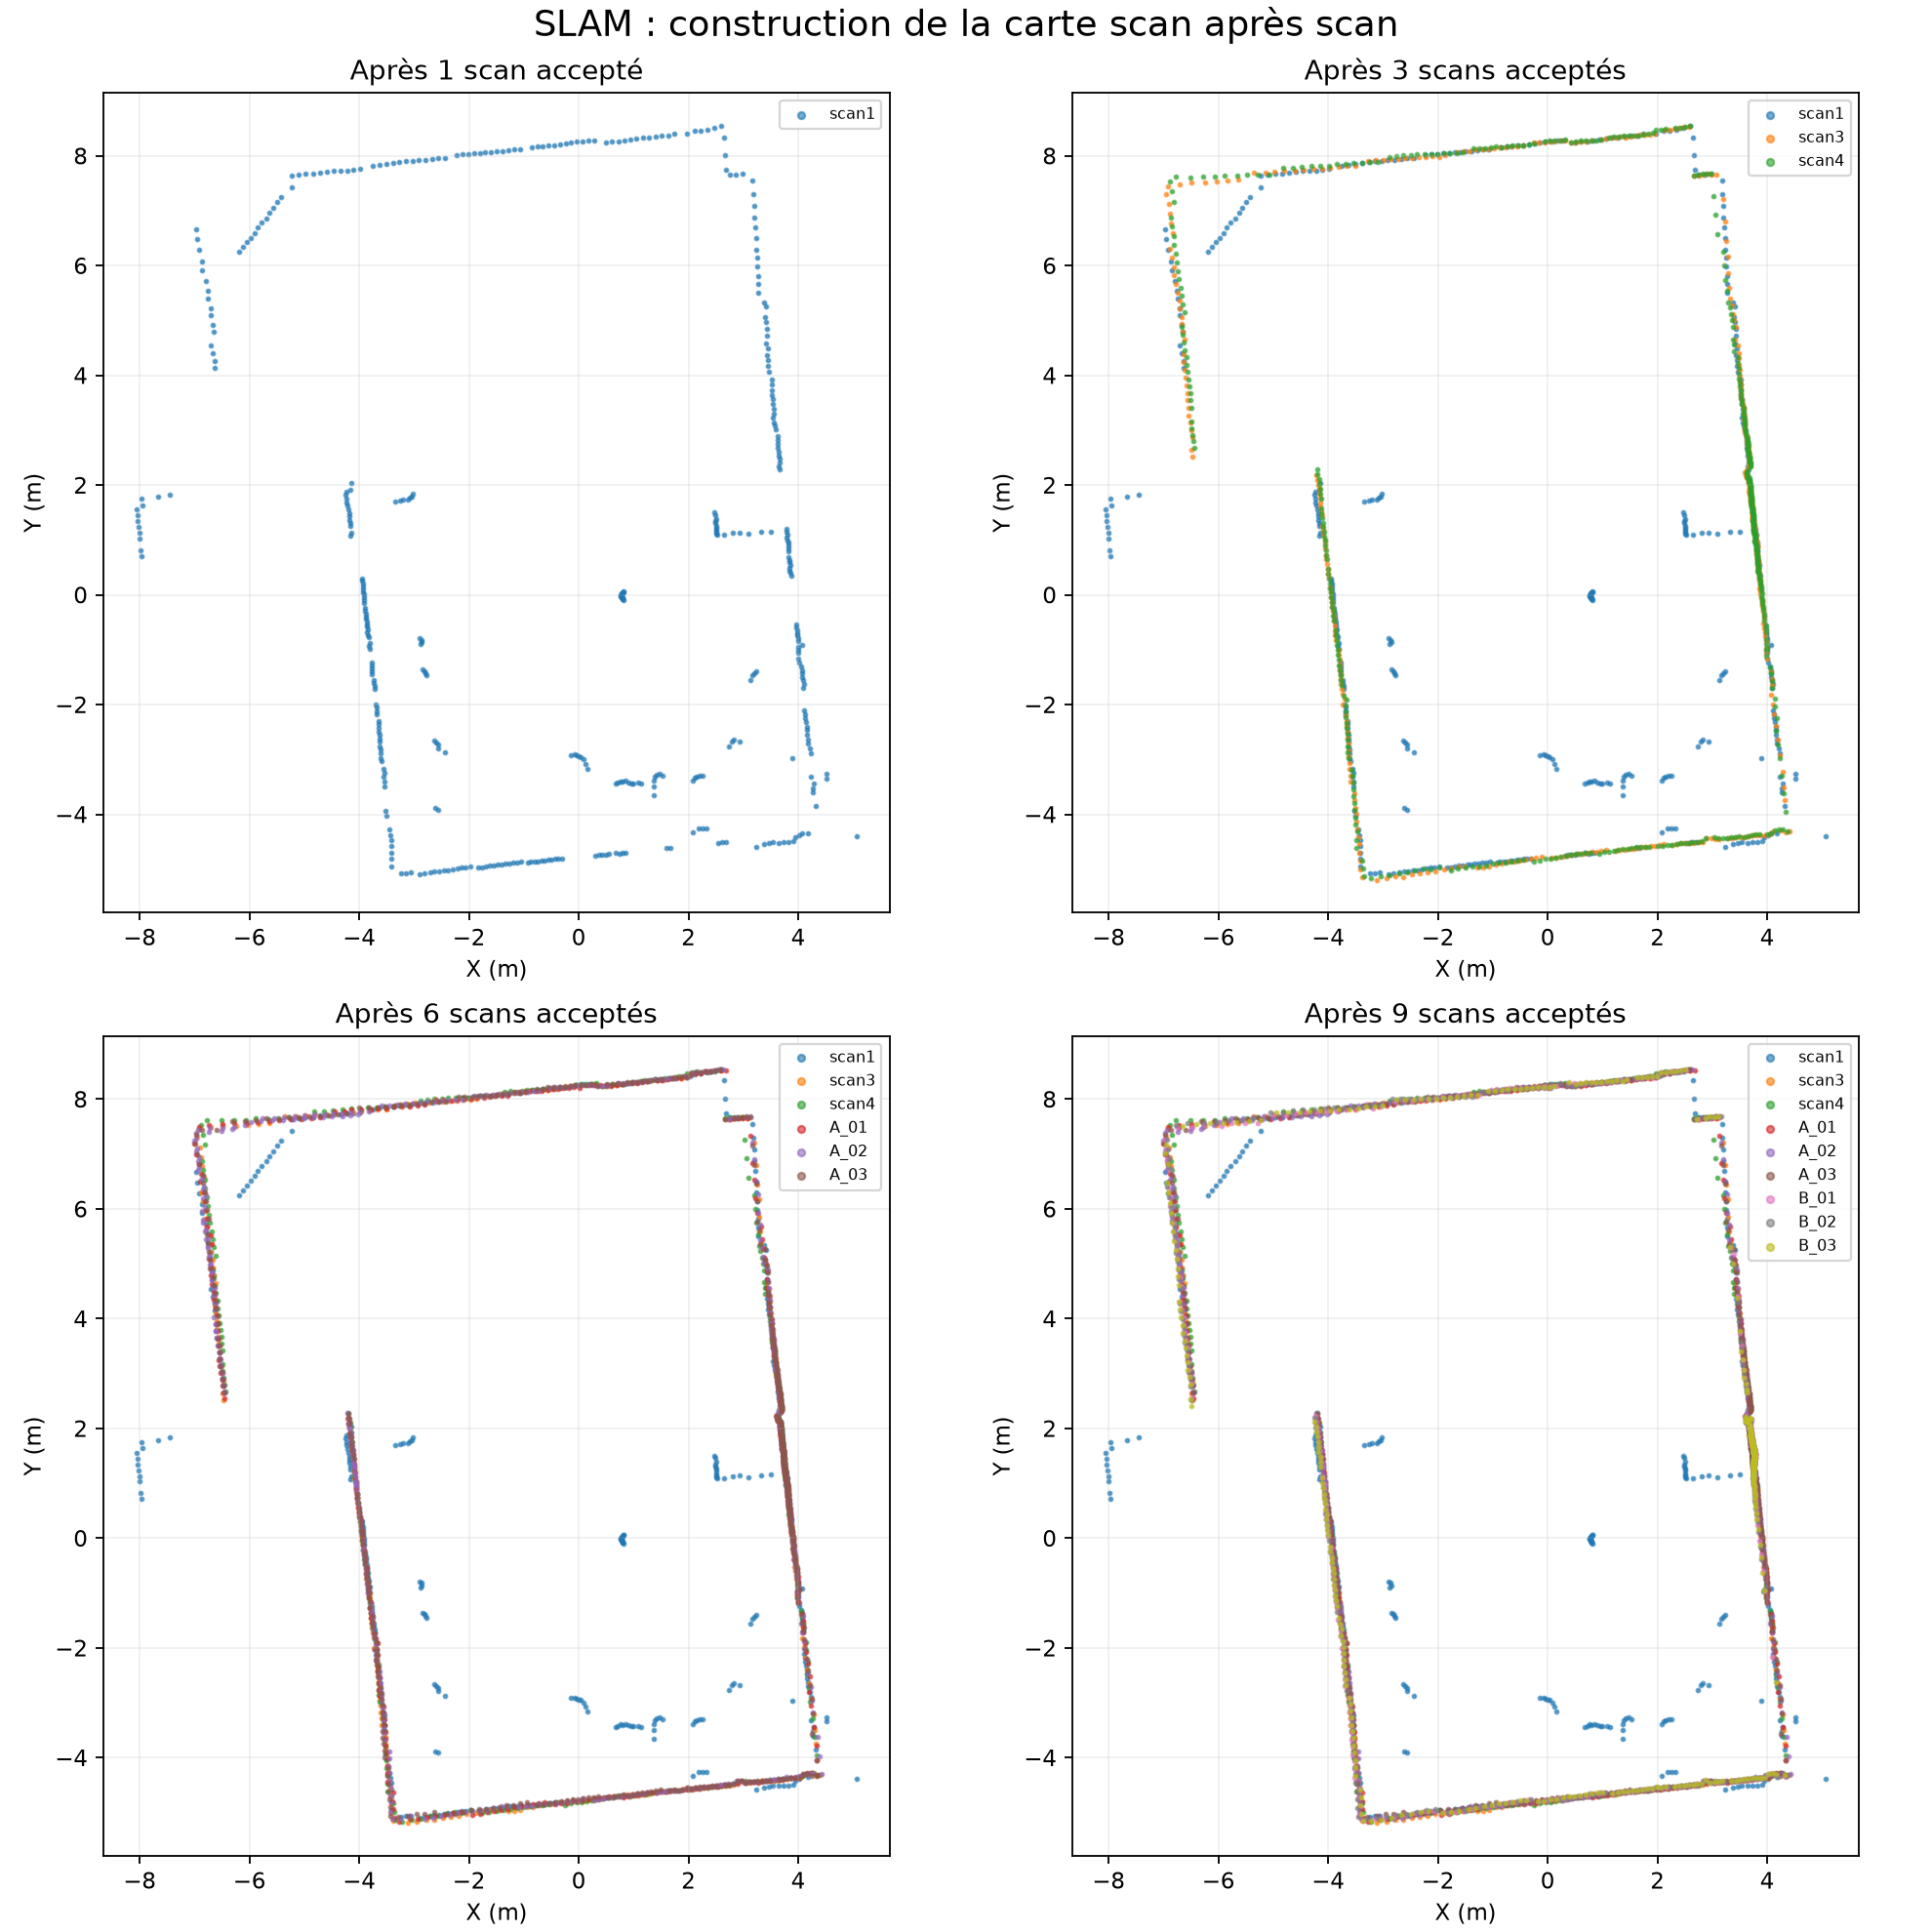
\includegraphics[width=0.90\textwidth]{../tp3/resultats/slam_progression_nuages.png}
\caption{Progression de la carte lors du rejeu incrémental des scans acceptés.}
\end{figure}

\begin{figure}[H]\centering
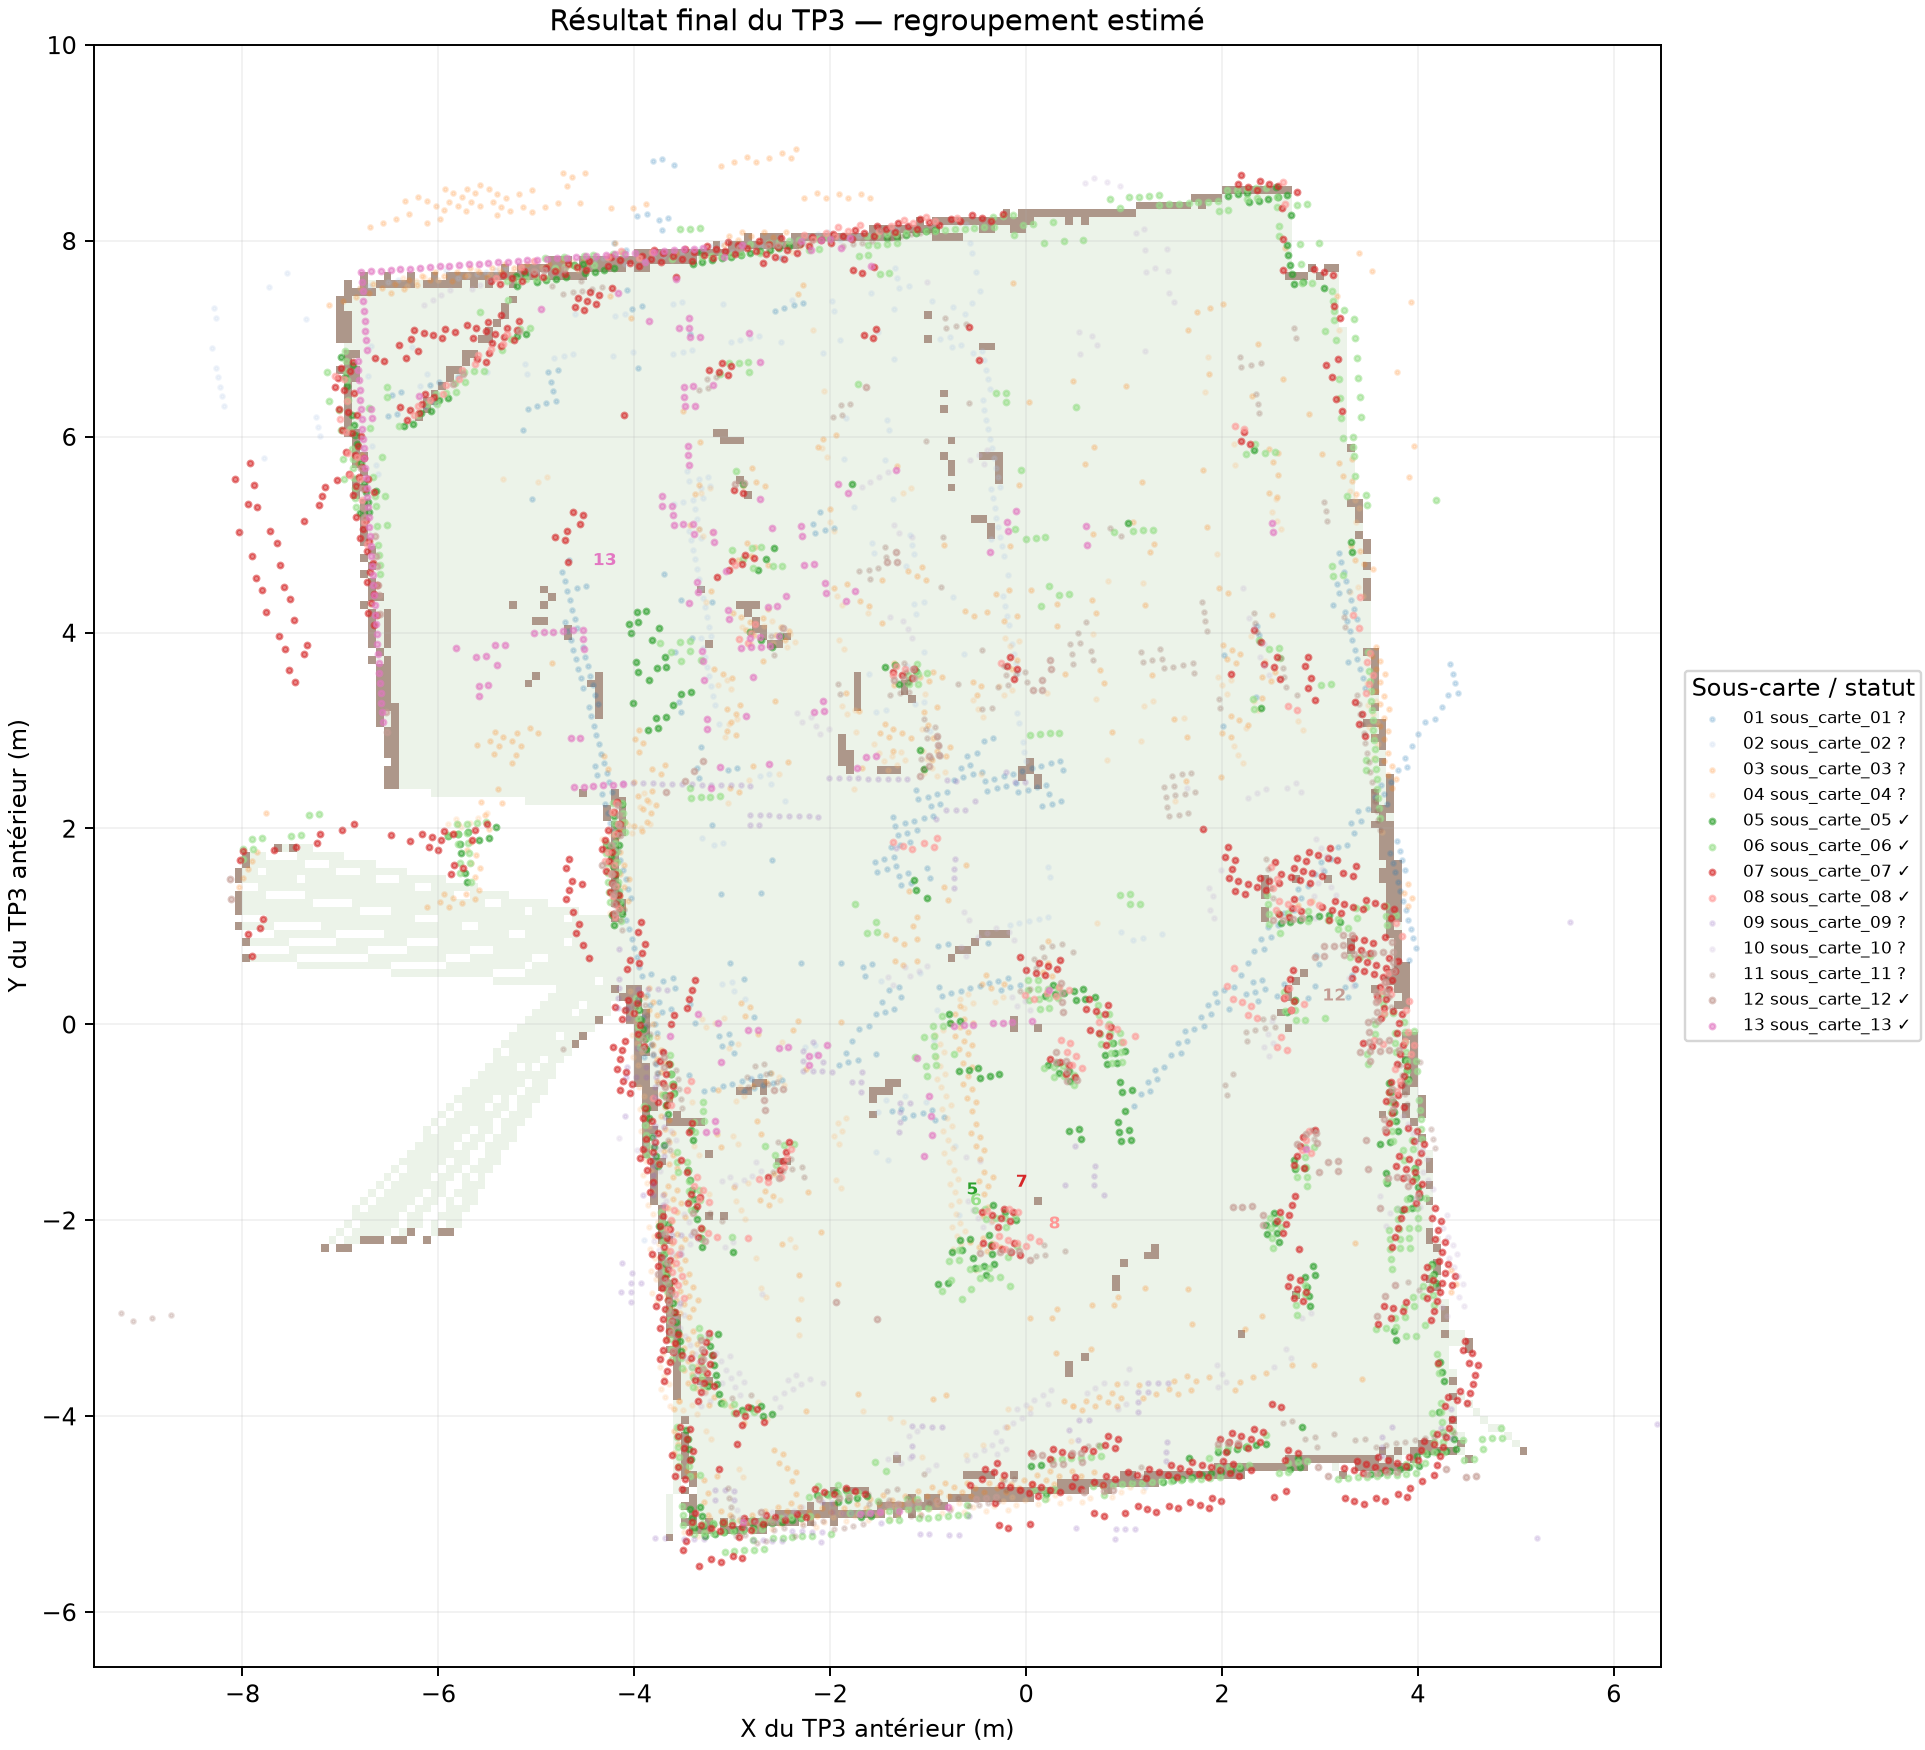
\includegraphics[width=0.80\textwidth]{../tp3/resultats/resultat_final.png}
\caption{Résultat final du TP3 : regroupement \emph{estimé} des sous-cartes et des scans du robot, sans validation métrique indépendante.}
\end{figure}

\subsection{Bonus : robot mobile et acquisitions LiDAR}
J'ai réussi à commander le déplacement du robot et à enregistrer des scans LiDAR pendant la séance de déplacement. Les outils du bonus comprennent le programme embarqué, l'interface d'acquisition, le rejeu des CSV, la construction de sous-cartes et une boucle de pilotage automatique par petites impulsions. Le dernier export cumulatif contient 114 scans ; en ajoutant les scans individuels sans compter un doublon, 117 acquisitions distinctes sont disponibles. Le contrôle de qualité en a accepté 86, réparties dans 13 sous-cartes. Parmi les raccords exploratoires entre sous-cartes, six passent les seuils indicatifs et sept restent incertains.

\begin{figure}[H]\centering
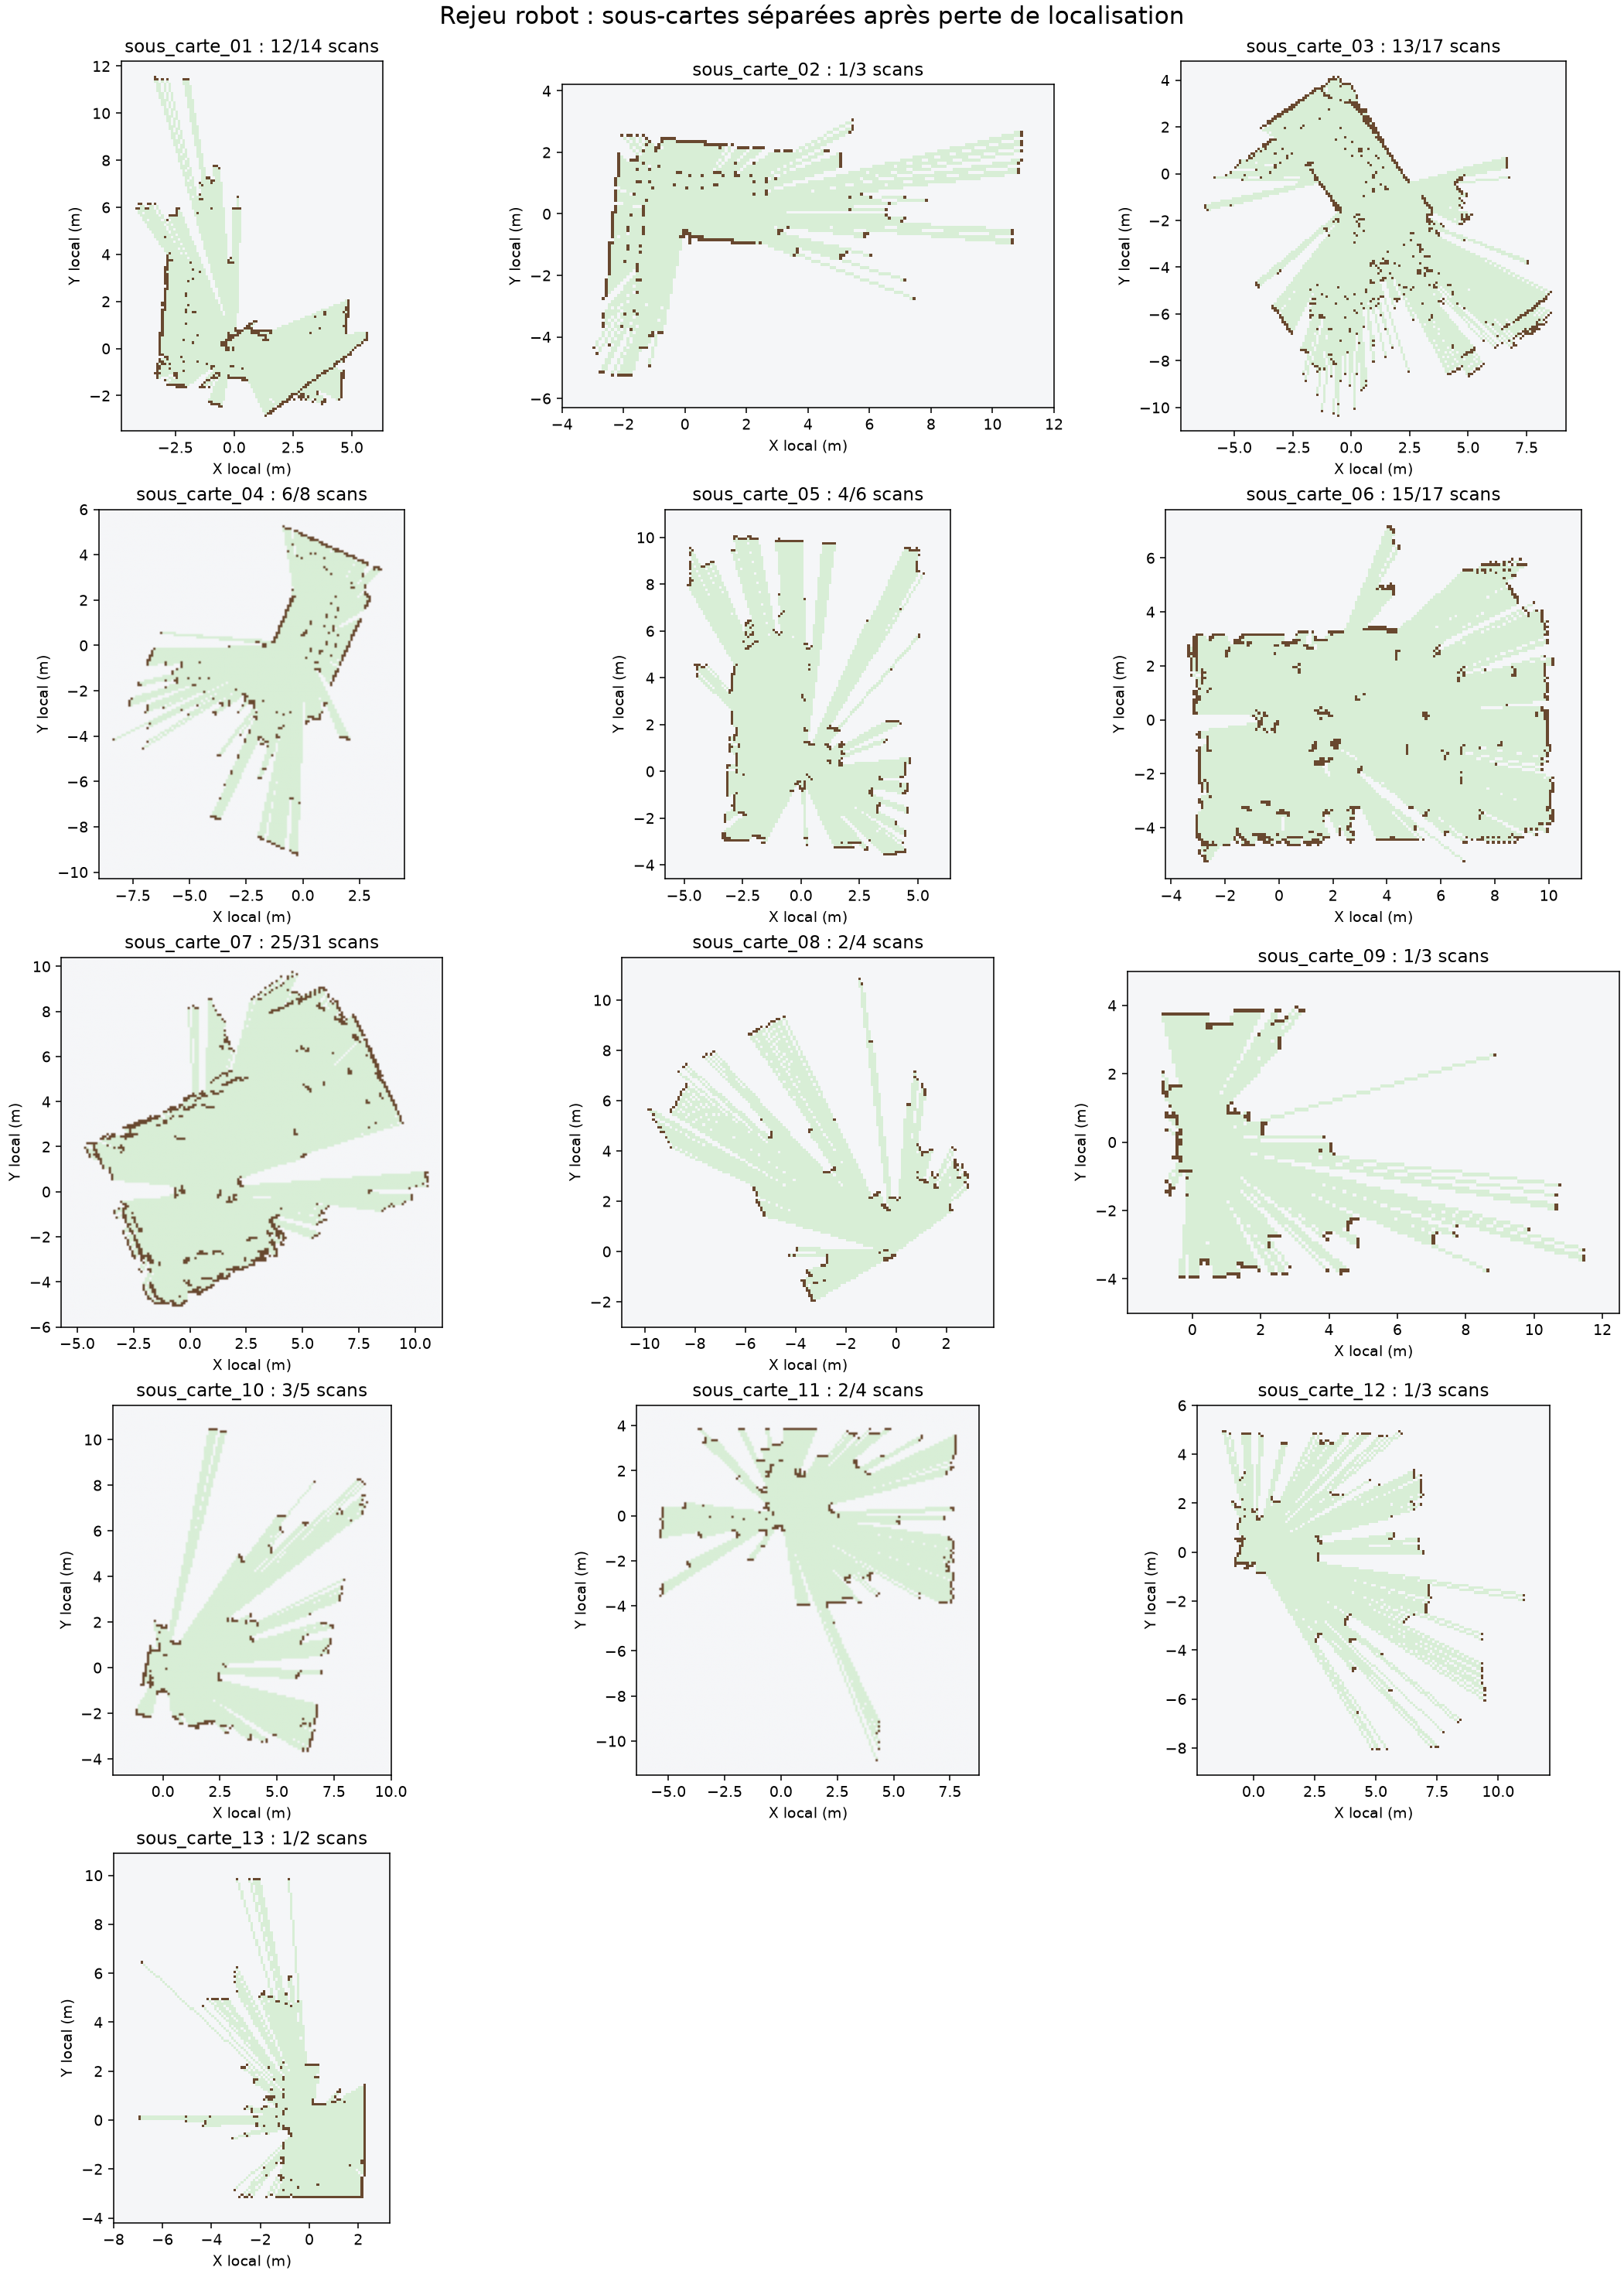
\includegraphics[width=0.83\textwidth]{../tp3/bonus_robot/resultats_rejeu/vue_sous_cartes.png}
\caption{Sous-cartes du robot mobile obtenues par recalage local des scans acceptés.}
\end{figure}

Il faut distinguer le déplacement du robot, qui a bien été réalisé, de la validation d'une cartographie LiDAR \emph{en continu pendant la rotation des roues}. Dans le code embarqué utilisé, la lecture LiDAR est interrompue pendant une impulsion moteur. Le pilotage automatique développé suit donc une séquence arrêt--scan--mise à jour--déplacement court. Son fonctionnement logiciel a été vérifié avec un faux robot, mais pas validé sur le robot physique. Par ailleurs, les champs de pose du CSV ne sont pas des mesures d'odométrie. La vue regroupée reste donc exploratoire : elle ne doit pas être présentée comme une carte complète et métriquement certifiée de la salle.

\section{Ce que je retiens personnellement}
\subsection{Ce que j'ai apprécié}
J'ai apprécié la progression du module : partir de valeurs d'angle et de distance, les voir devenir un nuage de points, puis une carte et enfin une estimation de pose rend les concepts concrets. Le moment où les scans acquis par mon propre robot ont commencé à former des murs reconnaissables a été particulièrement motivant. Les visualisations m'ont permis de comprendre rapidement les effets d'une erreur de rotation ou de translation. J'ai aussi apprécié de pouvoir confronter trois représentations différentes du même environnement, car elles ne mettent pas en évidence les mêmes informations.

L'aide du professeur, notamment à travers les documentations mises à notre disposition, a été utile pour avancer étape par étape. Les supports ne donnaient pas directement une carte correcte à partir de mes données : il fallait comprendre les hypothèses, les traduire en code et vérifier les choix sur les scans. C'est cette mise en pratique qui m'a le plus appris.

\subsection{Ce qui m'a paru difficile ou moins satisfaisant}
La partie la plus difficile a été d'obtenir des scans suffisamment comparables. Des changements de position, d'orientation, de hauteur ou de scène modifient fortement les correspondances. Les mêmes points peuvent sembler bien alignés à l'écran alors que la pose globale reste ambiguë. Il a également fallu surveiller les unités, le signe de l'axe $Y$, les doublons des exports cumulatifs et les zones invisibles. Ces détails prennent du temps, mais une erreur à ce niveau se propage dans toutes les cartes.

Je suis moins satisfait de l'absence de poses de référence mesurées lors des acquisitions réelles. Elle m'empêche de démontrer quantitativement l'erreur de localisation sur le robot, même lorsque la carte paraît convaincante. Les 100\,\% de succès de la simulation décrivent seulement les conditions de la simulation choisie. Le TP3 ne comporte pas non plus de fermeture de boucle ni d'optimisation globale : le recalage local peut donc accumuler une dérive.

\subsection{Ce que j'améliorerais}
Si je recommençais l'expérience, je préparerais un protocole d'acquisition plus rigoureux. Je fixerais et relèverais la hauteur du LiDAR, je marquerais plusieurs positions au sol, je mesurerais les déplacements et les angles avec leur incertitude, et je conserverais des scans de référence pris au même endroit. Cela permettrait de calculer des erreurs réelles, au lieu de se limiter aux résidus d'alignement. Je ferais aussi circuler le robot sur une trajectoire comportant un retour à une zone déjà vue afin d'essayer une fermeture de boucle.

Sur le plan technique, j'ajouterais une odométrie des roues et, si possible, une centrale inertielle pour fournir une prédiction de pose entre deux scans. Je testerais une mise à jour probabiliste de la grid map, un suivi de confiance des segments et une optimisation globale des sous-cartes. Enfin, je validerais physiquement la boucle de déplacement automatique sur un trajet court et contrôlé avant de l'étendre. Ces améliorations rendraient la carte plus fiable et l'évaluation plus convaincante.

\section{Conclusion}
Ce module m'a permis de relier l'acquisition, la géométrie, l'algorithmique et l'expérimentation sur un robot mobile. Je sais maintenant expliquer pourquoi une carte dépend à la fois des mesures du LiDAR et de la qualité des poses estimées. Les outils développés produisent des visualisations, une grid map, une carte vectorielle, trois méthodes de localisation évaluées en simulation et une première boucle de SLAM sur données enregistrées. Le robot a fourni de nouveaux scans pendant une séance de déplacement, avec un regroupement exploratoire de sous-cartes.

Le principal enseignement que j'en retiens est méthodologique : une carte visuellement plausible est un résultat intéressant, mais la validation de sa précision exige des mesures de référence indépendantes et une analyse des incertitudes. Les documentations du professeur m'ont aidé à bâtir cette démarche ; les limites observées sur mes propres données m'ont montré les étapes nécessaires pour aller vers un système de localisation et de cartographie plus robuste.

\end{document}
